\section{Příklad 2}
% Jako parametr zadejte skupinu (A-H)
\druhyZadani{H}

\begin{large}
\textbf{Riešenie:} (Metóda Théveninovej vety):\\
\end{large}

\textbf{·}
Začneme spočítaním sériovo zapojených rezistorov $R_4$ a $R_5$.

\begin{center}
$R_{45} = R_{4} + R_{5} = 205 + 560 = {765} \hspace{0,1cm} \SI{}{\ohm}$
\end{center}

\begin{figure}[h!]
    \centering
    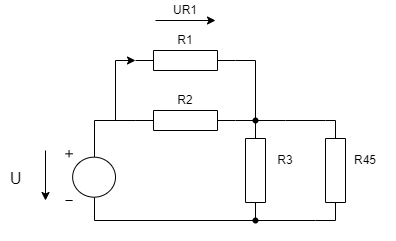
\includegraphics[width=0.5\textwidth]{IEL-Project/pictures/Pr2_1.png}
\end{figure}

\textbf{·}
Prekreslíme si obvod bez $R_1$ a nahradíme napätie zdroja „skratom“.

\begin{figure}[h!]
    \centering
    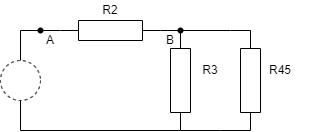
\includegraphics[width=0.35\textwidth]{IEL-Project/pictures/Pr2_2.png}
\end{figure}

\textbf{·}
Z obvodu vidíme, že rezistory $R_3$ a $R_{45}$ sú zapojené paralelne.

\begin{center}
$R_{345} = \frac{R_3 \cdot R_{45}}{R_3 + R_{45}} = \frac{580 \cdot 765}{580 + 765} = {329,8885} \hspace{0,1cm} \SI{}{\ohm}$
\end{center}

\begin{figure}[h!]
    \centering
    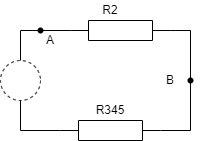
\includegraphics[width=0.35\textwidth]{IEL-Project/pictures/Pr2_3.png}
\end{figure}

\newpage

\textbf{·}
Spočítame si odpor $R_{AB} = R_i$ medzi bodmi A a B paralelnou úpravou rezistorov $R_2$ a $R_345$.

\begin{center}
$R_i = R_{AB} = \frac{R_2 \cdot R_{345}}{R_2 + R_{345}} = \frac{360 \cdot 329,8885}{360 + 329,8885}= {172,1436} \hspace{0,1cm} \SI{}{\ohm}$
\end{center}

\textbf{·}
V ďalšom kroku si obvod prekreslíme bez rezistoru $R_1$ a určíme napätie $U_i$ medzi bodmi A a B. Rezistory $R_1$ a $R_2$ sú zapojené paralelne, teda vieme povedať, že napätie na týchto rezistoroch je rovnaké.

\begin{center}
    $U_1 = U_i = U_2$
\end{center}

\begin{figure}[h!]
    \centering
    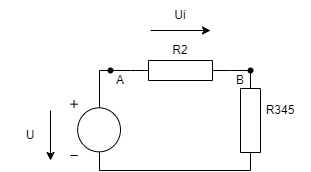
\includegraphics[width=0.4\textwidth]{IEL-Project/pictures/Pr2_4.png}
\end{figure}

\textbf{·}
Obvod zjednodušíme na rezistor $R_{2345}$ teda na $R_{EKV}$. Dostaneme ho sčítaním odporov rezistorov $R_2$ a $R_{345}$.

\begin{center}
    $R_{EKV} = R_{2345} = R_2 + R_{345} = 360 + 329,8885 = {689,8885} \hspace{0,1cm} \SI{}{\ohm}$
\end{center}

\begin{center}
    $I = \frac{U}{R_{EKV}} = \frac{220}{689,8885} = {0.3189}\hspace{0,1cm} \SI{}{\ampere}$
\end{center}

\begin{figure}[h!]
    \centering
    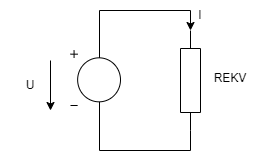
\includegraphics[width=0.4\textwidth]{IEL-Project/pictures/Pr2_5.png}
\end{figure}

\textbf{·}
Následne dopočítame napätie $U_1$ pomocou napätia $U_2$, ktoré je rovnaké. Po vypočítaní napätia $U_1$  dopočítame prúd $I_{R1}$.

\begin{center}
    $U_1 = U_2 = R_2 \cdot I = 360 \cdot 0,3189 = {114,804} \hspace{0,1cm} \SI{}{\volt}$
\end{center}

\begin{center}
    $I_{R1} = \frac{U_1}{R_1} = \frac{114,804}{190} = {0,6042} \hspace{0,1cm} \SI{}{\ampere}$
\end{center}